\documentclass[aspectratio=169]{beamer}

%\documentclass[handout]{beamer}
%% To make 4 per page
%\usepackage{pgfpages}
%\mode<handout>{\setbeamercolor{background canvas}{bg=white}}
%\pgfpagesuselayout{4 on 1}[letterpaper,landscape]%,border shrink=5mm]

\usetheme{default}
% Slide setup, colour independent

\usepackage{amsmath,amssymb,amsthm}
\usepackage{colortbl}
\usepackage{bm}
\usepackage{xcolor}
\usepackage{dsfont}
\usepackage{setspace}
%\usepackage{subfigure}
% To use \ding{234} and the like
\usepackage{pifont}
% To cross reference between slide files
\usepackage{zref-xr,zref-user}
% Use something like
% \zexternaldocument{fileI}
% in the tex files. And cite using \zref instead of \ref

% Fields and the like
\def\IC{\mathbb{C}}
\def\IF{\mathbb{F}}
\def\II{\mathbb{I}}
\def\IJ{\mathbb{J}}
\def\IM{\mathbb{M}}
\def\IN{\mathbb{N}}
\def\IP{\mathbb{P}}
\def\IR{\mathbb{R}}
\def\IZ{\mathbb{Z}}
\def\11{\mathds{1}}


% Bold lowercase
\def\ba{\mathbf{a}}
\def\bb{\mathbf{b}}
\def\bc{\mathbf{c}}
\def\bd{\mathbf{d}}
\def\be{\mathbf{e}}
\def\bf{\mathbf{f}}
\def\bh{\mathbf{h}}
\def\bi{\mathbf{i}}
\def\bj{\mathbf{j}}
\def\bk{\mathbf{k}}
\def\bn{\mathbf{n}}
\def\bp{\mathbf{p}}
\def\br{\mathbf{r}}
\def\bs{\mathbf{s}}
\def\bu{\mathbf{u}}
\def\bv{\mathbf{v}}
\def\bw{\mathbf{w}}
\def\bx{\mathbf{x}}
\def\by{\mathbf{y}}
\def\bz{\mathbf{z}}

% Bold capitals
\def\bB{\mathbf{B}}
\def\bD{\mathbf{D}}
\def\bF{\mathbf{F}}
\def\bG{\mathbf{G}}
\def\bI{\mathbf{I}}
\def\bL{\mathbf{L}}
\def\bN{\mathbf{N}}
\def\bP{\mathbf{P}}
\def\bR{\mathbf{R}}
\def\bS{\mathbf{S}}
\def\bT{\mathbf{T}}
\def\bX{\mathbf{X}}

% Bold numbers
\def\b0{\mathbf{0}}

% Bold greek
\bmdefine{\bmu}{\bm{\mu}}
\def\bphi{\bm{\phi}}
\def\bvarphi{\bm{\varphi}}

% Bold red sentence
\def\boldred#1{{\color{red}\textbf{#1}}}
\def\defword#1{{\color{orange}\textbf{#1}}}

% Caligraphic letters
\def\A{\mathcal{A}}
\def\B{\mathcal{B}}
\def\C{\mathcal{C}}
\def\D{\mathcal{D}}
\def\E{\mathcal{E}}
\def\F{\mathcal{F}}
\def\G{\mathcal{G}}
\def\H{\mathcal{H}}
\def\I{\mathcal{I}}
\def\L{\mathcal{L}}
\def\M{\mathcal{M}}
\def\N{\mathcal{N}}
\def\P{\mathcal{P}}
\def\R{\mathcal{R}}
\def\S{\mathcal{S}}
\def\T{\mathcal{T}}
\def\U{\mathcal{U}}
\def\V{\mathcal{V}}

% tt font for code
\def\code#1{{\tt #1}}

% i.e., e.g.
\def\eg{\emph{e.g.}}
\def\ie{\emph{i.e.}}


% Operators and special symbols
\def\nbOne{{\mathchoice {\rm 1\mskip-4mu l} {\rm 1\mskip-4mu l}
{\rm 1\mskip-4.5mu l} {\rm 1\mskip-5mu l}}}
\def\cov{\ensuremath{\mathsf{cov}}}
\def\Var{\ensuremath{\mathsf{Var}\ }}
\def\Im{\textrm{Im}\;}
\def\Re{\textrm{Re}\;}
\def\det{\ensuremath{\mathsf{det}}}
\def\diag{\ensuremath{\mathsf{diag}}}
\def\nullspace{\ensuremath{\mathsf{null}}}
\def\nullity{\ensuremath{\mathsf{nullity}}}
\def\rank{\ensuremath{\mathsf{rank}}}
\def\range{\ensuremath{\mathsf{range}}}
\def\sgn{\ensuremath{\mathsf{sgn}}}
\def\Span{\ensuremath{\mathsf{span}}}
\def\tr{\ensuremath{\mathsf{tr}}}
\def\imply{$\Rightarrow$}
\def\restrictTo#1#2{\left.#1\right|_{#2}}
\newcommand{\parallelsum}{\mathbin{\!/\mkern-5mu/\!}}
\def\dsum{\mathop{\displaystyle \sum }}%
\def\dind#1#2{_{\substack{#1\\ #2}}}

\DeclareMathOperator{\GL}{GL}
\DeclareMathOperator{\Rel}{Re}
\def\Nt#1{\left|\!\left|\!\left|#1\right|\!\right|\!\right|}
\newcommand{\tripbar}{|\! |\! |}



% The beamer bullet (in base colour)
\def\bbullet{\leavevmode\usebeamertemplate{itemize item}\ }

% Theorems and the like
\newtheorem{proposition}[theorem]{Proposition}
\newtheorem{property}[theorem]{Property}
\newtheorem{importantproperty}[theorem]{Property}
\newtheorem{importanttheorem}[theorem]{Theorem}
%\newtheorem{lemma}[theorem]{Lemma}
%\newtheorem{corollary}[theorem]{Corollary}
\newtheorem{remark}[theorem]{Remark}
\setbeamertemplate{theorems}[numbered]
%\setbeamertemplate{theorems}[ams style]

%
%\usecolortheme{orchid}
%\usecolortheme{orchid}

\def\red{\color[rgb]{1,0,0}}
\def\blue{\color[rgb]{0,0,1}}
\def\green{\color[rgb]{0,1,0}}


% Get rid of navigation stuff
\setbeamertemplate{navigation symbols}{}

% Set footline/header line
\setbeamertemplate{footline}
{%
\quad p. \insertpagenumber \quad--\quad \insertsection\vskip2pt
}
% \setbeamertemplate{headline}
% {%
% \quad\insertsection\hfill p. \insertpagenumber\quad\mbox{}\vskip2pt
% }


\makeatletter
\newlength\beamerleftmargin
\setlength\beamerleftmargin{\Gm@lmargin}
\makeatother

% Colours for special pages
\def\extraContent{yellow!20}


%%%%%%%%%%%%%%%%%
\usepackage{tikz}
\usetikzlibrary{shapes,arrows}
\usetikzlibrary{positioning}
\usetikzlibrary{shapes.symbols,shapes.callouts,patterns}
\usetikzlibrary{calc,fit}
\usetikzlibrary{backgrounds}
\usetikzlibrary{decorations.pathmorphing,fit,petri}
\usetikzlibrary{automata}
\usetikzlibrary{fadings}
\usetikzlibrary{patterns,hobby}

\usetikzlibrary{backgrounds,fit,petri}


\usepackage{pgfplots}
\pgfplotsset{compat=1.6}
\pgfplotsset{ticks=none}

\usetikzlibrary{decorations.markings}
\usetikzlibrary{arrows.meta}
\tikzset{>=stealth}

% For tikz
\usetikzlibrary{shapes,arrows}
\usetikzlibrary{positioning}
\tikzstyle{cloud} = [draw, ellipse,fill=red!20, node distance=0.87cm,
minimum height=2em]
\tikzstyle{line} = [draw, -latex']


%%% For max frame images
\newenvironment{changemargin}[2]{%
\begin{list}{}{%
\setlength{\topsep}{0pt}%
\setlength{\leftmargin}{#1}%
\setlength{\rightmargin}{#2}%
\setlength{\listparindent}{\parindent}%
\setlength{\itemindent}{\parindent}%
\setlength{\parsep}{\parskip}%
}%
\item[]}{\end{list}}


% Make one image take up the entire slide content area in beamer,.:
% centered/centred full-screen image, with title:
% This uses the whole screen except for the 1cm border around it
% all. 128x96mm
\newcommand{\titledFrameImage}[2]{
\begin{frame}{#1}
%\begin{changemargin}{-1cm}{-1cm}
\begin{center}
\includegraphics[width=108mm,height=\textheight,keepaspectratio]{#2}
\end{center}
%\end{changemargin}
\end{frame}
}

% Make one image take up the entire slide content area in beamer.:
% centered/centred full-screen image, no title:
% This uses the whole screen except for the 1cm border around it
% all. 128x96mm
\newcommand{\plainFrameImage}[1]{
\begin{frame}[plain]
%\begin{changemargin}{-1cm}{-1cm}
\begin{center}
\includegraphics[width=108mm,height=76mm,keepaspectratio]{#1}
\end{center}
%\end{changemargin}
\end{frame}
}

% Make one image take up the entire slide area, including borders, in beamer.:
% centered/centred full-screen image, no title:
% This uses the entire whole screen
\newcommand{\maxFrameImage}[1]{
\begin{frame}[plain]
\begin{changemargin}{-1cm}{-1cm}
\begin{center}
\includegraphics[width=\paperwidth,height=\paperheight,keepaspectratio]
{#1}
\end{center}
\end{changemargin}
\end{frame}
}

% This uses the entire whole screen (to include in frame)
\newcommand{\maxFrameImageNoFrame}[1]{
\begin{changemargin}{-1cm}{-1cm}
\begin{center}
\includegraphics[width=\paperwidth,height=0.99\paperheight,keepaspectratio]
{#1}
\end{center}
\end{changemargin}
}

% Make one image take up the entire slide area, including borders, in beamer.:
% centered/centred full-screen image, no title:
% This uses the entire whole screen
\newcommand{\maxFrameImageColor}[2]{
\begin{frame}[plain]
\setbeamercolor{normal text}{bg=#2!20}
\begin{changemargin}{-1cm}{-1cm}
\begin{center}
\includegraphics[width=\paperwidth,height=\paperheight,keepaspectratio]
{#1}
\end{center}
\end{changemargin}
\end{frame}
}


\usepackage{tikz}
\usetikzlibrary{patterns,hobby}
\usepackage{pgfplots}
\pgfplotsset{compat=1.6}
\pgfplotsset{ticks=none}

\usetikzlibrary{backgrounds}
\usetikzlibrary{decorations.markings}
\usetikzlibrary{arrows.meta}
\tikzset{>=stealth}

\tikzset{
  clockwise arrows/.style={
    postaction={
      decorate,
      decoration={
        markings,
        mark=between positions 0.1 and 0.9 step 40pt with {\arrow{>}},
   }}}}


   %%%%%%%%%%%
% To have links to parts in the outline
\makeatletter
\AtBeginPart{%
  \addtocontents{toc}{\protect\beamer@partintoc{\the\c@part}{\beamer@partnameshort}{\the\c@page}}%
}
%% number, shortname, page.
\providecommand\beamer@partintoc[3]{%
  \ifnum\c@tocdepth=-1\relax
    % requesting onlyparts.
    \makebox[6em]{Part #1:} \textcolor{green!30!blue}{\hyperlink{#2}{#2}}
    \par
  \fi
}
\define@key{beamertoc}{onlyparts}[]{%
  \c@tocdepth=-1\relax
}
\makeatother%

\newcommand{\nameofthepart}{}
\newcommand{\nupart}[1]%
    {   \part{#1}%
        \renewcommand{\nameofthepart}{#1}%
        {
          \setbeamercolor{background canvas}{bg=orange!50}
          \begin{frame}{#1}%\partpage 
          \hypertarget{\nameofthepart}{}\tableofcontents%
          \end{frame}
        }
    }



\usecolortheme{orchid}

%% Listings
\usepackage{listings}
\definecolor{mygreen}{rgb}{0,0.6,0}
\definecolor{mygray}{rgb}{0.5,0.5,0.5}
\definecolor{mymauve}{rgb}{0.58,0,0.82}
\definecolor{mygold}{rgb}{1,0.843,0}
\definecolor{myblue}{rgb}{0.537,0.812,0.941}

\definecolor{lgreen}{rgb}{0.6,0.9,.6}
\definecolor{lred}{rgb}{1,0.5,.5}

\lstloadlanguages{R}
\lstset{ %
  language=R,
  backgroundcolor=\color{black!05},   % choose the background color
  basicstyle=\footnotesize\ttfamily,        % size of fonts used for the code
  breaklines=true,                 % automatic line breaking only at whitespace
  captionpos=b,                    % sets the caption-position to bottom
  commentstyle=\color{mygreen},    % comment style
  escapeinside={\%*}{*)},          % if you want to add LaTeX within your code
  keywordstyle=\color{red},       % keyword style
  stringstyle=\color{mygold},     % string literal style
  keepspaces=true,
  columns=fullflexible,
  tabsize=4,
}
% Could also do (in lstset)
% basicstyle==\fontfamily{pcr}\footnotesize
\lstdefinelanguage{Renhanced}%
  {keywords={abbreviate,abline,abs,acos,acosh,action,add1,add,%
      aggregate,alias,Alias,alist,all,anova,any,aov,aperm,append,apply,%
      approx,approxfun,apropos,Arg,args,array,arrows,as,asin,asinh,%
      atan,atan2,atanh,attach,attr,attributes,autoload,autoloader,ave,%
      axis,backsolve,barplot,basename,besselI,besselJ,besselK,besselY,%
      beta,binomial,body,box,boxplot,break,browser,bug,builtins,bxp,by,%
      c,C,call,Call,case,cat,category,cbind,ceiling,character,char,%
      charmatch,check,chol,chol2inv,choose,chull,class,close,cm,codes,%
      coef,coefficients,co,col,colnames,colors,colours,commandArgs,%
      comment,complete,complex,conflicts,Conj,contents,contour,%
      contrasts,contr,control,helmert,contrib,convolve,cooks,coords,%
      distance,coplot,cor,cos,cosh,count,fields,cov,covratio,wt,CRAN,%
      create,crossprod,cummax,cummin,cumprod,cumsum,curve,cut,cycle,D,%
      data,dataentry,date,dbeta,dbinom,dcauchy,dchisq,de,debug,%
      debugger,Defunct,default,delay,delete,deltat,demo,de,density,%
      deparse,dependencies,Deprecated,deriv,description,detach,%
      dev2bitmap,dev,cur,deviance,off,prev,,dexp,df,dfbetas,dffits,%
      dgamma,dgeom,dget,dhyper,diag,diff,digamma,dim,dimnames,dir,%
      dirname,dlnorm,dlogis,dnbinom,dnchisq,dnorm,do,dotplot,double,%
      download,dpois,dput,drop,drop1,dsignrank,dt,dummy,dump,dunif,%
      duplicated,dweibull,dwilcox,dyn,edit,eff,effects,eigen,else,%
      emacs,end,environment,env,erase,eval,equal,evalq,example,exists,%
      exit,exp,expand,expression,External,extract,extractAIC,factor,%
      fail,family,fft,file,filled,find,fitted,fivenum,fix,floor,for,%
      For,formals,format,formatC,formula,Fortran,forwardsolve,frame,%
      frequency,ftable,ftable2table,function,gamma,Gamma,gammaCody,%
      gaussian,gc,gcinfo,gctorture,get,getenv,geterrmessage,getOption,%
      getwd,gl,glm,globalenv,gnome,GNOME,graphics,gray,grep,grey,grid,%
      gsub,hasTsp,hat,heat,help,hist,home,hsv,httpclient,I,identify,if,%
      ifelse,Im,image,\%in\%,index,influence,measures,inherits,install,%
      installed,integer,interaction,interactive,Internal,intersect,%
      inverse,invisible,IQR,is,jitter,kappa,kronecker,labels,lapply,%
      layout,lbeta,lchoose,lcm,legend,length,levels,lgamma,library,%
      licence,license,lines,list,lm,load,local,locator,log,log10,log1p,%
      log2,logical,loglin,lower,lowess,ls,lsfit,lsf,ls,machine,Machine,%
      mad,mahalanobis,make,link,margin,match,Math,matlines,mat,matplot,%
      matpoints,matrix,max,mean,median,memory,menu,merge,methods,min,%
      missing,Mod,mode,model,response,mosaicplot,mtext,mvfft,na,nan,%
      names,omit,nargs,nchar,ncol,NCOL,new,next,NextMethod,nextn,%
      nlevels,nlm,noquote,NotYetImplemented,NotYetUsed,nrow,NROW,null,%
      numeric,\%o\%,objects,offset,old,on,Ops,optim,optimise,optimize,%
      options,or,order,ordered,outer,package,packages,page,pairlist,%
      pairs,palette,panel,par,parent,parse,paste,path,pbeta,pbinom,%
      pcauchy,pchisq,pentagamma,persp,pexp,pf,pgamma,pgeom,phyper,pico,%
      pictex,piechart,Platform,plnorm,plogis,plot,pmatch,pmax,pmin,%
      pnbinom,pnchisq,pnorm,points,poisson,poly,polygon,polyroot,pos,%
      postscript,power,ppoints,ppois,predict,preplot,pretty,Primitive,%
      print,prmatrix,proc,prod,profile,proj,prompt,prop,provide,%
      psignrank,ps,pt,ptukey,punif,pweibull,pwilcox,q,qbeta,qbinom,%
      qcauchy,qchisq,qexp,qf,qgamma,qgeom,qhyper,qlnorm,qlogis,qnbinom,%
      qnchisq,qnorm,qpois,qqline,qqnorm,qqplot,qr,Q,qty,qy,qsignrank,%
      qt,qtukey,quantile,quasi,quit,qunif,quote,qweibull,qwilcox,%
      rainbow,range,rank,rbeta,rbind,rbinom,rcauchy,rchisq,Re,read,csv,%
      csv2,fwf,readline,socket,real,Recall,rect,reformulate,regexpr,%
      relevel,remove,rep,repeat,replace,replications,report,require,%
      resid,residuals,restart,return,rev,rexp,rf,rgamma,rgb,rgeom,R,%
      rhyper,rle,rlnorm,rlogis,rm,rnbinom,RNGkind,rnorm,round,row,%
      rownames,rowsum,rpois,rsignrank,rstandard,rstudent,rt,rug,runif,%
      rweibull,rwilcox,sample,sapply,save,scale,scan,scan,screen,sd,se,%
      search,searchpaths,segments,seq,sequence,setdiff,setequal,set,%
      setwd,show,sign,signif,sin,single,sinh,sink,solve,sort,source,%
      spline,splinefun,split,sqrt,stars,start,stat,stem,step,stop,%
      storage,strstrheight,stripplot,strsplit,structure,strwidth,sub,%
      subset,substitute,substr,substring,sum,summary,sunflowerplot,svd,%
      sweep,switch,symbol,symbols,symnum,sys,status,system,t,table,%
      tabulate,tan,tanh,tapply,tempfile,terms,terrain,tetragamma,text,%
      time,title,topo,trace,traceback,transform,tri,trigamma,trunc,try,%
      ts,tsp,typeof,unclass,undebug,undoc,union,unique,uniroot,unix,%
      unlink,unlist,unname,untrace,update,upper,url,UseMethod,var,%
      variable,vector,Version,vi,warning,warnings,weighted,weights,%
      which,while,window,write,\%x\%,x11,X11,xedit,xemacs,xinch,xor,%
      xpdrows,xy,xyinch,yinch,zapsmall,zip},%
   otherkeywords={!,!=,~,$,*,\%,\&,\%/\%,\%*\%,\%\%,<-,<<-,_,/},%
   alsoother={._$},%
   sensitive,%
   morecomment=[l]\#,%
   morestring=[d]",%
   morestring=[d]'% 2001 Robert Denham
  }%

%%%%%%% 
%% Definitions in yellow boxes
\usepackage{etoolbox}
\setbeamercolor{block title}{use=structure,fg=structure.fg,bg=structure.fg!40!bg}
\setbeamercolor{block body}{parent=normal text,use=block title,bg=block title.bg!20!bg}

\BeforeBeginEnvironment{definition}{%
	\setbeamercolor{block title}{fg=black,bg=yellow!20!white}
	\setbeamercolor{block body}{fg=black, bg=yellow!05!white}
}
\AfterEndEnvironment{definition}{
	\setbeamercolor{block title}{use=structure,fg=structure.fg,bg=structure.fg!20!bg}
	\setbeamercolor{block body}{parent=normal text,use=block title,bg=block title.bg!50!bg, fg=black}
}
\BeforeBeginEnvironment{importanttheorem}{%
	\setbeamercolor{block title}{fg=black,bg=red!20!white}
	\setbeamercolor{block body}{fg=black, bg=red!05!white}
}
\AfterEndEnvironment{importanttheorem}{
	\setbeamercolor{block title}{use=structure,fg=structure.fg,bg=structure.fg!20!bg}
	\setbeamercolor{block body}{parent=normal text,use=block title,bg=block title.bg!50!bg, fg=black}
}
\BeforeBeginEnvironment{importantproperty}{%
	\setbeamercolor{block title}{fg=black,bg=red!50!white}
	\setbeamercolor{block body}{fg=black, bg=red!30!white}
}
\AfterEndEnvironment{importantproperty}{
	\setbeamercolor{block title}{use=structure,fg=structure.fg,bg=structure.fg!20!bg}
	\setbeamercolor{block body}{parent=normal text,use=block title,bg=block title.bg!50!bg, fg=black}
}


% Beginning of a section
\AtBeginSection[]{
	{
		\setbeamercolor{background canvas}{bg=yellow!10}
		\begin{frame}[noframenumbering,plain]
			\framesubtitle{\nameofthepart Chapter \insertromanpartnumber \ -- \iteminsert{\insertpart}}
			\tableofcontents[
				currentsection,
				sectionstyle=show/shaded,
				subsectionstyle=show/show/hide]
		\end{frame}
	\addtocounter{page}{-1}
	%\addtocounter{framenumber}{-1} 
	}
}

% Beginning of a section
\AtBeginSubsection[]{
	{
		\setbeamercolor{background canvas}{bg=green!10}
		\begin{frame}[noframenumbering,plain]
				\framesubtitle{\nameofthepart Chapter \insertromanpartnumber \ -- \iteminsert{\insertpart}}
				\tableofcontents[
					currentsection,
					sectionstyle=show/show,
					currentsubsection,
					subsectionstyle=show/shaded/hide]
			\end{frame}
		\addtocounter{page}{-1}
	}
}

% To cross reference from other slide files
\zexternaldocument{MATH-4370-7370-slides-03-eigenpairs-similarity}
\zexternaldocument{MATH-4370-7370-slides-06-nonnegative-matrices}

% To have theorems and everything derived prefixed by the slide set
% number
\renewcommand{\thetheorem}{7.\arabic{theorem}}

\title{A worked out example using matrices}
\author{Julien Arino}
\date{Fall 2023}

%%%%%%%%%%%%%%%%%%%%%
%%%%%%%%%%%%%%%%%%%%%
%%%%%%%%%%%%%%%%%%%%%
%%%%%%%%%%%%%%%%%%%%%
%%%%%%%%%%%%%%%%%%%%%
%%%%%%%%%%%%%%%%%%%%%
%%%%%%%%%%%%%%%%%%%%%
%%%%%%%%%%%%%%%%%%%%%
\begin{document}

% The title page
\begin{frame}[noframenumbering,plain]
  \begin{tikzpicture}[remember picture,overlay]
    \node[above right,inner sep=0pt] at (current page.south west)
    {
        
\includegraphics[width=\paperwidth]{title-page-picture.png}
    };
\end{tikzpicture}
	\titlepage
\end{frame}
\addtocounter{page}{-1}
  
  
\begin{frame}{Outline}
	  \tableofcontents[hideallsubsections]
\end{frame}
\addtocounter{page}{-1}


%%%%%%%%%%%%%%%%%%%%%%%%%%%
%%%%%%%%%%%%%%%%%%%%%%%%%%%
%%%%%%%%%%%%%%%%%%%%%%%%%%%
%%%%%%%%%%%%%%%%%%%%%%%%%%%


%%%%%%%%%%%%%%%%%%
%%%%%%%%%%%%%%%%%%
%%%%%%%%%%%%%%%%%%
%%%%%%%%%%%%%%%%%%
\section{Position of the problem}
\begin{frame}{Rael \& Taylor (2018)}
	{\footnotesize\emph{A flow network model for animal movement on a landscape with application to invasion}, Theoretical Ecology}
	\vfill
	\[
	P_i' = P_iB(P_i)+\sum_{j=1}^N 
	a_{ji}P_jm(P_j,P_i)
	-P_i\sum_{j=1}^N a_{ij}m(P_i,P_j)
	\]
	where
	\[
	m(P_i, P_j) = \frac{\max\{0, \pi(P_i)-\pi(P_j)\}}{d_{ij}}
	\qquad \pi(P_i) = \frac{P_i}{K_i}
	\]
	$d_{ij}$ distance from $i$ to $j$, $K_i$ carrying capacity
	\[
	B(P_i) = \begin{cases}
	r_i\left(1-\dfrac{P_i}{K_i}\right) & \textrm{sources} \\
	-r_i & \textrm{sinks}
	\end{cases}
	\]
\end{frame}
	
	
\begin{frame}{Position of the problem}
	Assume a metapopulation of patches connected through transport of individuals between them
	\vfill
	Some patches are sources, others are sinks:
	\begin{itemize}
		\item Population tends to persist in sources
		\item Population tends to vanish in sinks
	\end{itemize}
	\vfill
	\emph{Ceteris paribus}, does there exist a ratio of the number of source to sink patches s.t. the population of the coupled system persists?
\end{frame}

\begin{frame}{Something like this...}
    \begin{center}
        \begin{tikzpicture}
            \node[inner sep=-30pt] (sink1) at (0,0)
                {
\includegraphics[width=.3\textwidth]{FIGS/sink-patch.png}};
                \node[inner sep=-30pt] (sink2) at (5.5,-1.25)
                {
\includegraphics[width=.3\textwidth]{FIGS/sink-patch.png}};
                \node[inner sep=-30pt] (source1) at (8,2)
                {
\includegraphics[width=.3\textwidth]{FIGS/source-patch.png}};
                \node[inner sep=-30pt] (source2) at (9.5,-2)
                {
\includegraphics[width=.3\textwidth]{FIGS/source-patch.png}};
                \node[inner sep=-30pt] (source3) at (3.5,1.5)
                {
\includegraphics[width=.3\textwidth]{FIGS/source-patch.png}};
				\path [line, very thick, bend right=5] (sink1) to (sink2);
				\path [line, very thick, bend right=25] (sink1) to (source2);
				\path [line, very thick, bend right=25] (sink2) to (source3);
				\path [line, very thick, bend right=25] (source2) to (source3);
				\path [line, very thick, bend right=25] (source1) to (source3);
				\path [line, very thick, bend right=25] (source3) to (sink1);
        \end{tikzpicture}
    \end{center}
\end{frame}


\begin{frame}
	\textbf{Obvious special cases}
\end{frame}

\begin{frame}{This is not good}
    \begin{center}
        \begin{tikzpicture}
            \node[inner sep=-30pt] (sink1) at (0,0)
                {
\includegraphics[width=.3\textwidth]{FIGS/sink-patch.png}};
                \node[inner sep=-30pt] (sink2) at (5.5,-1.25)
                {
\includegraphics[width=.3\textwidth]{FIGS/sink-patch.png}};
                \node[inner sep=-30pt] (source1) at (8,2)
                {
\includegraphics[width=.3\textwidth]{FIGS/sink-patch.png}};
                \node[inner sep=-30pt] (source2) at (9.5,-2)
                {
\includegraphics[width=.3\textwidth]{FIGS/sink-patch.png}};
                \node[inner sep=-30pt] (source3) at (3.5,1.5)
                {
\includegraphics[width=.3\textwidth]{FIGS/sink-patch.png}};
				\path [line, very thick, bend right=5] (sink1) to (sink2);
				\path [line, very thick, bend right=25] (sink1) to (source2);
				\path [line, very thick, bend right=25] (sink2) to (source3);
				\path [line, very thick, bend right=25] (source2) to (source3);
				\path [line, very thick, bend right=25] (source1) to (source3);
				\path [line, very thick, bend right=25] (source3) to (sink1);
        \end{tikzpicture}
    \end{center}
\end{frame}

\begin{frame}{This probably is}
    \begin{center}
        \begin{tikzpicture}
            \node[inner sep=-30pt] (sink1) at (0,0)
                {
\includegraphics[width=.3\textwidth]{FIGS/source-patch.png}};
                \node[inner sep=-30pt] (sink2) at (5.5,-1.25)
                {
\includegraphics[width=.3\textwidth]{FIGS/source-patch.png}};
                \node[inner sep=-30pt] (source1) at (8,2)
                {
\includegraphics[width=.3\textwidth]{FIGS/source-patch.png}};
                \node[inner sep=-30pt] (source2) at (9.5,-2)
                {
\includegraphics[width=.3\textwidth]{FIGS/source-patch.png}};
                \node[inner sep=-30pt] (source3) at (3.5,1.5)
                {
\includegraphics[width=.3\textwidth]{FIGS/source-patch.png}};
				\path [line, very thick, bend right=5] (sink1) to (sink2);
				\path [line, very thick, bend right=25] (sink1) to (source2);
				\path [line, very thick, bend right=25] (sink2) to (source3);
				\path [line, very thick, bend right=25] (source2) to (source3);
				\path [line, very thick, bend right=25] (source1) to (source3);
				\path [line, very thick, bend right=25] (source3) to (sink1);
        \end{tikzpicture}
    \end{center}
\end{frame}



\section[Sources-sinks model]{A metapopulation of sources and sinks with explicit movement}

\begin{frame}{Model for $N$ patches}
	W.l.o.g.: $S\geq 0$ first patches are sources, $N-S$ remaining are sinks [w.l.o.g. but not that trivial nonetheless]
	\vfill
	\textbf{Sources:}
	\begin{subequations}\label{sys:simple_model}
	\begin{equation}
	P_i' = r_iP_i\left(1-\frac{P_i}{K_i}\right)+\sum_{j=1}^N m_{ij}P_j,
	\quad i=1,\ldots,S
	\end{equation}
	\vfill
	\textbf{Sinks:}
	\begin{equation}
	P_i' = -r_iP_i +\sum_{j=1}^N m_{ij}P_j,\quad i=S+1,\ldots,N
	\end{equation}
	\end{subequations}
	\vfill
	\[
	m_{ii} = -\sum_{\substack{j=1\\j\neq i}}^N m_{ji}
	\]
\end{frame}	
	

\begin{frame}{Vector form (v1)}
	$\bP=(P_1,\ldots,P_N)^T$
	\vfill
	\[
	\bP' = \bG(\bP)\bP+\M\bP
	\]
	where
	\[
	\bG(\bP) =
	\diag\left(
	r_1\left(1-\frac{P_1}{K_1}\right),\ldots,r_S\left(1-\frac{P_S}{K_S}\right),
	-r_{S+1},\ldots,-r_N
	\right)
	\]
	\[
	\M =
	\begin{pmatrix}
	-\sum\limits_{\substack{j=1\\j\neq 1}}^N m_{j1} & m_{12} & \cdots & m_{1N} \\
	m_{21} & -\sum\limits_{\substack{j=1\\j\neq 2}}^N m_{j2} & \cdots & m_{2N} \\
	& & \ddots & \\
	m_{N1} & m_{N2} & \cdots & -\sum\limits_{\substack{j=1\\j\neq N}}^N m_{jN}
	\end{pmatrix}
	\]
\end{frame}
	
\begin{frame}{Vector form (v2)}
	$\bP_s=(P_1,\ldots,P_S)^T$ (sources), \quad $\bP_t =(P_{S+1},\ldots,P_N)$ (sinks)
	\vfill
	\begin{align*}
	\bP_s' &= \bG_s(\bP_s)\bP_s+\M_s\bP_s+\M_{st}\bP_t \\
	\bP_t' &= -\D_t\bP_t+\M_{ts}\bP_s+\M_t\bP_t
	\end{align*}
	where
	\[
	\bG_s(\bP_s) =
	\diag\left(
	r_1\left(1-\frac{P_1}{K_1}\right),\ldots,r_S\left(1-\frac{P_S}{K_S}\right)
	\right)
	\]
	\[
	\D_t = \diag\left(r_{S+1},\ldots,r_N\right)
	\]
	\[
	\begin{pmatrix}
	\M_s & \M_{st} \\ \M_{ts} & \M_t
	\end{pmatrix} = \M
	\]
\end{frame}


\begin{frame}{Main result we want to get to}
	\begin{theorem}\label{th:main_result}
		$\exists$ a unique critical interval $\S_{int}\subset(0,N)\subset\IR$ s.t. if the number of source patches $S<\min(\S_{int})$, the population-free equilibrium (PFE) $(P_1,\ldots,P_N)=(0,\ldots,0)$ of \eqref{sys:simple_model} is locally asymptotically stable and if $S>\max(\S_{int})$, the PFE is unstable
		\vskip0.5cm
		If, additionally, the digraph of patches is strongly connected, then $\S_{int}$ reduces to a single point $S^c$ and the PFE is globally asymptotically stable in the case that $S<S^c$; in the case that $S>S^c$, there is a unique component-wise positive equilibrium $\bP^*$ that is GAS with respect to $\IR_+^N\setminus\{0\}$
		\end{theorem}
		
\end{frame}


%%%%%%%%%%%%%%%%%%
%%%%%%%%%%%%%%%%%%
%%%%%%%%%%%%%%%%%%
%%%%%%%%%%%%%%%%%%
\section{The movement matrix}
\begin{frame}{Properties of the movement matrix $\M$}
	\begin{lemma}\label{lemma:mvt_matrix}
		\begin{enumerate}
			\item $0\in\sigma(\M)$ corresponding to left e.v. $\11^T$ \hfill[$\sigma$ spectrum] \label{lemma:mvt_matrix_0ev}
			\item $-\M$ is a singular M-matrix \label{lemma:mvt_matrix_MMmatrix}
			\item $0=s(\M)\in\sigma(\M)$ \hfill[$s$ spectral abscissa] \label{lemma:mvt_matrix_SB_eq0}
			\item If $\M$ irreducible, then $s(\M)$ has multiplicity 1 \label{lemma:mvt_matrix_SB_mult1}
		\end{enumerate}
	\end{lemma}
\end{frame}



\begin{frame}{Proof of Lemma~\ref{lemma:mvt_matrix}}
\ref{lemma:mvt_matrix_0ev}. The result is obvious: all column sums of $\M$ equal zero, i.e., $\nbOne^T\M=0\nbOne^T$
\vfill
\noindent\ref{lemma:mvt_matrix_SB_eq0}. Using the Gershgorin Disk Theorem \cite{Varga2010} on $\M$ indicates that all Gershgorin disks are tangent to the imaginary axis at $(0,0)$. As 0 is an eigenvalue of $\M$, it follows that $s(\M)=0$
\vfill
\noindent\ref{lemma:mvt_matrix_SB_mult1}. This is a direct consequence of using the Perron-Frobenius Theorem on the essentially nonnegative matrix $\M$
\end{frame}

\begin{frame}{Proof of Lemma~\ref{lemma:mvt_matrix} (cont'd)}
	\noindent\ref{lemma:mvt_matrix_MMmatrix}. 
	From the Gershgorin Disk Theorem \cite{Varga2010}, all eigenvalues of $-\M$ belong to disks that lie to the right of the imaginary axis and, from the zero column sums, are tangent to that axis at $(0,0)$
	\vfill
	Now consider $-\M+\varepsilon\II$, for $\varepsilon>0$. 
	This shifts the centers of all Gershgorin disks to the right by $\varepsilon$ \cite[Problem 1.2.P8]{HornJohnson2013} but does not change their radii, so all disks now lie strictly to the right of the imaginary axis 
	\vfill
	Thus all eigenvalues of $-\M+\varepsilon\II$ have positive real parts
	\vfill
	Furthermore, $-\M$ and $-\M+\varepsilon\II$ are of class $Z_n$: they have nonpositive offdiagonal entries. 
	As a consequence, by \cite[Theorem 5.1.1(18)]{Fiedler2008}, $-\M+\varepsilon\II$ is of class $K$, i.e., an M-matrix.
	Since this is true for all $\varepsilon>0$, \cite[Theorem 5.2.1(1)]{Fiedler2008} implies that $-\M$ is of class $K_0$. 
	So $-\M$ is an M-matrix and it is singular
\end{frame}

\begin{frame}{Properties of the movement matrix $\M$ (cont'd)}
	\begin{proposition}[$D$ a diagonal matrix]\label{prop:perturbation_mvtMatrix}
		\begin{enumerate}
			\item $s(\M+d\II)=d$, $\forall d\in\IR$ \label{prop:perturbation_mvtMatrix_d}
			\item $s(\M+D)\in\sigma(\M+D)$ associated to $\bv>\b0$. If $\M$ irreducible, $s(\M+D)$ has  multiplicity 1 and is associated to $\bv\gg \b0$ \label{prop:perturbation_mvtMatrix_D}
			\item If $\diag (D)\gg \b0$, then $D-\M$ invertible M-matrix and $(D-\M)^{-1}> \b0$ \label{prop:perturbation_mvtMatrix_DmM1}
			\item $\M$ irreducible and $\diag(D)>\b0$ $\Longrightarrow$ $D-\M$ nonsingular irreducible M-matrix and $(D-\M)^{-1}\gg \b0$ \label{prop:perturbation_mvtMatrix_DmM2}
		\end{enumerate}
	\end{proposition}
\end{frame}


\begin{frame}{Proof of Proposition~\ref{prop:perturbation_mvtMatrix}}
\ref{prop:perturbation_mvtMatrix_d}. From Lemma~\ref{lemma:mvt_matrix}(\ref{lemma:mvt_matrix_SB_eq0}), $s(\M)=0$. Therefore, using a ``spectrum shift'' \cite[Problem 1.2.P8]{HornJohnson2013}, $s(\M+d\II)=d$
\vfill
\noindent\ref{prop:perturbation_mvtMatrix_D}. These are direct consequences of applying the Perron-Frobenius Theorem to the essentially nonnegative matrix $\M+D$
\vfill
\end{frame}


\begin{frame}{Proof of Proposition~\ref{prop:perturbation_mvtMatrix} (cont'd)}
\noindent\ref{prop:perturbation_mvtMatrix_DmM1}.
Define $\underline{d}=\min_{i=1,\ldots,N}d_{ii}$. $\diag (D)\gg \b0$ $\implies$ $\underline{d}>0$ $\implies$ $-\M\leq d\II-\M\leq D-\M$. From \cite[Theorem 5.2.5]{Fiedler2008}, $d\II-\M$ is an M-matrix. 
Since $s(\M)=0$, using a ``spectrum shift'' \cite[Problem 1.2.P8]{HornJohnson2013}, all eigenvalues of $d\II-\M$ have real parts larger
than $\underline{d}$, so $\underline{d}\II-\M$ is a nonsingular M-matrix. 
In turn, \cite[Theorem 5.1.1(4)]{Fiedler2008} $\implies$ $D-\M$ nonsingular M-matrix and \cite[Theorem 5.1.1(11)]{Fiedler2008} leads to the conclusion
\vfill
\noindent\ref{prop:perturbation_mvtMatrix_DmM2}. 
Suppose that $\M$ is irreducible. 
Let $\overline{d}=\max_{i=1,\ldots,N}d_{ii}>0$.
Then $D-\M$ is  irreducible and diagonally dominant with all columns $k=1,\ldots,N$ such that $d_{kk}=\overline{d}$ satisfying the strict diagonal
dominance requirement. (Other columns with nonzero entries in $D$ also satisfy the requirement.)
As a consequence, \cite[Theorem 1.11]{Varga2010} implies that $D-\M$ is nonsingular and inverse positivity follows from \cite[Theorem 5.2.10]{Fiedler2008}
\end{frame}

\begin{frame}{$-\M$ is also the Laplacian matrix of a digraph}
Note that $-\M$ is also the Laplacian matrix of a directed graph
\vfill 
As such, finer estimates of the location of eigenvalues are available; see, e.g.,  \cite{AgaevChebotarev2005}
\vfill
However, the main concern here is with the spectral abscissa, so this is not needed
\end{frame}


%%%%%%%%%%%%%%%%%%
%%%%%%%%%%%%%%%%%%
%%%%%%%%%%%%%%%%%%
%%%%%%%%%%%%%%%%%%
\section{Local analysis of the model}
\begin{frame}{The \emph{population-free equilibrium} (PFE)}
	We find the PFE
	$\bP_s=\bP_t=\b0$ 
	\vfill
	At the PFE,
	\begin{equation}\label{eq:J_PFE}
	J_{\textrm{PFE}}^S = \M+(\D_s\oplus -\D_t)
	\end{equation}
	where $\D_s=\bG_s(\b0)=\diag(r_1,\ldots,r_S)$
	\vfill
	The matrix
	\[
	\D_s\oplus -\D_t=\diag (r_1,\ldots,r_S,-r_{S+1},\ldots,-r_N)
	\]
	has $S$ diagonal entries $>0$ and $N-S$ diagonal entries $<0$
\end{frame}


\begin{frame}{Mechanism of the existence proof}
	Start with $S=0$ (only sinks)
	\newline
	$\implies$ $\D_s$ vacuous and $\D_s\oplus -\D_t = \diag(-r_1,\ldots,-r_N)$ \newline
	$\implies$ $s(J_{PFE}^S)<0$
	\vfill
	Finish with $S=N$ (only sources)
	\newline
	$\implies$ $\D_t$ vacuous and $\D_s\oplus -\D_t = \diag(r_1,\ldots,r_N)$ \newline
	$\implies$ $s(J_{PFE}^S)>0$
	\vfill
	Eigenvalues of $J_{\textrm{PFE}}^S$ depend continuously of entries of $J_{\textrm{PFE}}^S$, so $s(J_{\textrm{PFE}}^S)$ changes signs, we are done.. if we are happy with a lot of uncertainty about behaviour of $s(J_{\textrm{PFE}}^S)$
\end{frame}


\begin{frame}{Continuous perturbation of the spectrum}
	\underline{For $S\in\{0,\ldots,N-1\}$}
	\[
	J_{\textrm{PFE}}^{S,\varepsilon} =
	\M+\diag(r_1,\ldots,r_S,\varepsilon,-r_{S+2},\ldots,-r_N)
	\]
	where $\varepsilon\in[-r_{S+1},r_{S+1}]$ is in $(S+1)^{\textrm{th}}$ position
	\vfill
	\underline{For $S\in[0,N]$}
	\begin{equation}\label{eq:xi_epsilon_ri}
	J_{\textrm{PFE}}^{S}=J_{\textrm{PFE}}^{\xi,\varepsilon},
	\quad\textrm{with}\quad
	\xi=\lfloor S\rfloor,
	\quad 
	\varepsilon= 2(S-\lfloor S\rfloor)r_i-r_i
	\end{equation}
	where $i=\lfloor S\rfloor+1$ if $S<N$ and $i=N$ when $S=N$
	\vfill
	\underline{Generally} we vary $\zeta$ continuously in each $[-r_{S+1},r_{S+1}]$
	\[
	J_{\textrm{PFE}}^{S,-r_{S+1}} = J_{\textrm{PFE}}^{S}
	\quad\textrm{and}\quad
	J_{\textrm{PFE}}^{S,r_{S+1}} = J_{\textrm{PFE}}^{S+1}
	\]
\end{frame}

\begin{frame}{The spectral abscissa $s(J_{\textrm{PFE}}^S)$ switches signs}
	\begin{lemma}\label{lemma:S_nonzero_at_ends}
		Let $\underline{r}=\min\limits_{i=1,\ldots, N} \{r_i\}$
		\vskip0.5cm
		Then $s(J_{\textrm{PFE}}^0) \leq -\underline{r} <0$ and  $s(J_{\textrm{PFE}}^N)\geq \underline{r} >0$
	\end{lemma}
\end{frame}

\begin{frame}{Proof of Lemma~\ref{lemma:S_nonzero_at_ends}}
	If $S=0$, then
	\[
	J_{\textrm{PFE}}^0=\M+\diag (-r_1,\ldots,-r_N)
	\]
	\vfill
	From Proposition~\ref{lemma:mvt_matrix}(\ref{lemma:mvt_matrix_SB_eq0}), $s(\M) = 0$. 
	Note that this follows from using the Gershgorin Theorem, where for $\M$, all Gershgorin disks are left of the imaginary axis and tangent to origin of the complex plane
	\vfill
	Then the centres of the Gershorin disks of $\M+\diag (-r_1,\ldots,-r_N)$ are shifted left by $r_1,\ldots,r_N$ while the radii remain the same
	\vfill
	As a consequence, the closest disk(s) to the origin of the complex plane have centre(s) $-\underline{r}$ and thus $s(\M+\diag (-r_1,\ldots,-r_N))\leq-\underline{r}<0$
\end{frame}

\begin{frame}{Proof of Lemma~\ref{lemma:S_nonzero_at_ends} (cont'd)}
	If $S=N$, then
	\[
	J_{\textrm{PFE}}^N=\M+\diag (r_1,\ldots,r_N)
	\]
	\vfill
	For $i=1,\ldots,N$, define $e_i=r_i-\underline{r}\geq 0$, then
	\[
	J_{\textrm{PFE}}^N=\M+\underline{r}\II+\diag (e_1,\ldots,e_N)
	\]
	where, by Proposition~\ref{prop:perturbation_mvtMatrix}(\ref{prop:perturbation_mvtMatrix_d}), $s(\M+\underline{r}\II)=\underline{r}>0$
\end{frame}

\begin{frame}{Proof of Lemma~\ref{lemma:S_nonzero_at_ends} (cont'd)}
	First, assume $\M$ irreducible
	\vfill
	Then $J_{\textrm{PFE}}^N$ is an irreducible essentially nonnegative matrix
	\vfill
	Since $J_{\textrm{PFE}}^N\geq \M+\underline{r}\II$, \cite[Corollary 4.3.2(3)]{Smith1995} $\implies$
	\[
		s(J_{\textrm{PFE}}^N)\geq s(\M+\underline{r}\II)=\underline{r}
	\]
	with the inequalities being strict if there exists at least one $e_i>0$
\end{frame}

\begin{frame}{Proof of Lemma~\ref{lemma:S_nonzero_at_ends} (cont'd)}
	Now assume that $\M$ reducible
	\vfill
	Then $\exists$ permutation matrix $P$ such that $P^T\M P$ is block upper triangular with irreducible blocks on the diagonal
	\vfill
	Call $C$ the number of such blocks, i.e., the number of strong components in the digraph of patches
	\vfill
	For $i=1,\ldots,C$, denote $n(i)$ the number of patches in strong component $i$ and $k(1),\ldots,k(n(i))$ their indices
	\vfill
	By abuse of notation, denote $\M_{ii}$ the corresponding diagonal block in the reduced form of $\M$
\end{frame}

\begin{frame}{Proof of Lemma~\ref{lemma:S_nonzero_at_ends} (cont'd)}
	Applying the permutation matrix $P$ to $J_{\textrm{PFE}}^N$ gives a block upper triangular matrix $P^TJ_{\textrm{PFE}}^NP$ with, for $i=1,\ldots,C$, the $n(i)\times n(i)$ diagonal blocks $\M_{ii}+E_i$ being irreducible and with
	\[
	E_i = \underline{r}\II
	+\diag\left(e_{k(1)},\ldots,e_{k(n(i))}\right)
	\]
\end{frame}


\begin{frame}{Proof of Lemma~\ref{lemma:S_nonzero_at_ends} (cont'd)}
	Fix $i=1,\ldots,C$ and let $\bv$ be a positive right eigenvector of $\M_{ii}+E_i$ corresponding to the spectral abscissa $s_1$ and $\bw$ be a positive left eigenvector of $\M_{ii}+\underline{r}\II$ corresponding to the spectral abscissa $s_2$.
	Then
	\begin{align*}
	s_1\bw^T\bv &= 
	\bw^T\left(\M_{ii}+\underline{r}\II +\diag(e_{k(1)},\ldots,e_{k(n(i))})\right)\bv \\
	&= \bw^T (\M_{ii}+\underline{r}\II)\bv + \bw^T \diag(e_{k(1)},\ldots,e_{k(n(i))})\bv \\
	&= s_2\bw^T\bv +\bw^T \diag(e_{k(1)},\ldots,e_{k(n(i))})\bv \\
	&\geq s_2\bw^T\bv
	\end{align*}
	the inequality being strict if at least one of the $e_{k(j)}$, $j=1,\ldots,n(i)$, is positive.
	Hence $s_1\geq s_2$, i.e., $s(\M_{ii}+E_i)\geq s(\M_{ii}+\underline{r}\II)$. 
	This is true for all diagonal blocks. Now, since $P^TJ_{\textrm{PFE}}^N P$ is block upper triangular, 
	\[
	s(J_{\textrm{PFE}}^N)=s(P^TJ_{\textrm{PFE}}^N P) =
	\max\{s(\M_{11}+E_1),\ldots,s(\M_{CC}+E_C)\}
	\]
\end{frame}

\begin{frame}{Proof of Lemma~\ref{lemma:S_nonzero_at_ends} (cont'd)}
	As $P^T(\M+\underline{r}\II)P$ is also block upper triangular,
	\[
	\underline{r} = s(\M+\underline{r}\II) =
	\max\{s(\M_{11}+\underline{r}\II),
	\ldots,
	s(\M_{11}+\underline{r}\II)\}
	\]
	As a consequence, $s(J_{\textrm{PFE}}^N)\geq \underline{r}>0$
\end{frame}

\begin{frame}
	Thus, $S^c$ necessarily lies in the open interval $(0,N)$.
	The following lemma is of interest and the method of proof of the second assertion is used again later
	\vfill
	\begin{lemma}\label{lemma:Mness_of_Jinterval}
	\begin{enumerate}
		\item \label{lemma:Mness_of_Jinterval_bounds}
		For all $S\in(0,N)\subset\IR$,
		\begin{equation}\label{ineq:bounds_J}
		J_{\textrm{PFE}}^{0}< J_{\textrm{PFE}}^{S}<
		J_{\textrm{PFE}}^{N}
		\end{equation}
		\item \label{lemma:Mness_of_Jinterval_increase}
		$J_{\textrm{PFE}}^{S}$ is an increasing function of $S$, in the sense that
	\begin{equation}\label{eq:J_increasing}
	\forall S_1,S_2\in[0,N]\subset\IR\textrm{ such that }S_1<S_2,
	\quad
	J_{\textrm{PFE}}^{S_1}< J_{\textrm{PFE}}^{S_2}
	\end{equation}
	%\item For all $S\in[0,S^c)$, $-J_{\textrm{PFE}}^{S}$ is a nonsingular M-matrix. The matrix $-J_{\textrm{PFE}}^{S}$ is a singular M-matrix.
	\end{enumerate}
	\end{lemma}
\end{frame}


\begin{frame}{Proof of Lemma~\ref{lemma:Mness_of_Jinterval}}
\ref{lemma:Mness_of_Jinterval_bounds}.
	Let $S\in(0,N)$ be fixed.
	Using \eqref{eq:xi_epsilon_ri}, this gives a pair $(\xi,\varepsilon)\in\{0,\ldots,N\}\times[-r_i,r_i]$, for $i=1\ldots N$, such that $J_{\textrm{PFE}}^{S}=J_{\textrm{PFE}}^{\xi,\varepsilon}$.
	We have
	\begin{align*}
	J_{\textrm{PFE}}^{\xi,\varepsilon}-J_{\textrm{PFE}}^{0} 
	&= \M+\diag(r_1,\ldots,r_{\xi},\varepsilon,-r_{\xi+2},\ldots,-r_N) \\
	&\quad -\M-\diag(-r_1,\ldots,-r_N) \\
	&= \diag(2r_1,\ldots,2r_{\xi},\varepsilon+r_{\xi+1},0,\ldots,0) \\
	&>\b0,
	\end{align*}
	since $\varepsilon\in[-r_{\xi+1},r_{\xi+1}]$. 
	Computing $J_{\textrm{PFE}}^{N}-J_{\textrm{PFE}}^{\xi,\varepsilon}$ at the other endpoint works similarly, giving \eqref{ineq:bounds_J}. 
\end{frame}

\begin{frame}{Proof of Lemma~\ref{lemma:Mness_of_Jinterval} (cont'd)}
	\ref{lemma:Mness_of_Jinterval_increase}. Use \eqref{eq:xi_epsilon_ri} again to obtain two pairs $(\xi_1,\varepsilon_1)$ and $(\xi_2,\varepsilon_2)$, where, by the assumption $S_1<S_2$, $\xi_1\leq\xi_2$. First, assume that $\xi_1<\xi_2$. Then
	\begin{align*}
	J_{\textrm{PFE}}^{\xi_2,\varepsilon_2}-J_{\textrm{PFE}}^{\xi_1,\varepsilon_1} 
	&= \diag(r_1,\ldots,r_{\xi_2},\varepsilon_2,-r_{\xi_2+2},\ldots,-r_N) \\
	&\quad -
	\diag(r_1,\ldots,r_{\xi_1},\varepsilon_1,-r_{\xi_1+2},\ldots,-r_N) \\
	&= \diag(0,\ldots,0,r_{\xi_1+1}-\varepsilon_1,
	2r_{\xi_1+2},
	\ldots,
	2r_{\xi_2},\varepsilon_2+r_{\xi_2+1},0,\ldots,0) \\
	&>\b0
	\end{align*}
	since $\varepsilon_1 \in[-r_{\xi_1+1},r_{\xi_1+1}],$ and $\varepsilon_2\in[-r_{\xi_2+1},r_{\xi_2+1}]$. Now assume $\xi_1=\xi_2$. Then, since $S_1<S_2$, we find that $\varepsilon_1<\varepsilon_2$ and the diagonal matrix in the subtraction $J_{\textrm{PFE}}^{\xi_2,\varepsilon_2}-J_{\textrm{PFE}}^{\xi_2,\varepsilon_1}$ takes the form $\diag(0,\ldots,0,\varepsilon_2-\varepsilon_1,0,\ldots,0)>\b0$. So \eqref{eq:J_increasing} holds
\end{frame}


\begin{frame}
	\begin{proposition}\label{prop:spectral_abs_increasing}
		$\M$ reducible $\implies$ $s(J_{\textrm{PFE}}^S)$ nondecreasing for $S\in[0,N]$
		\vskip0.2cm
		$\M$ irreducible $\implies$ $s(J_{\textrm{PFE}}^S)$ increasing for $S\in[0,N]$
	\end{proposition}
	\vfill
	$\implies$ $\exists \S_{int}\subset(0,N)$ (resp. $S^c\in(0,N)$) s.t. PFE LAS if $S<\min(\S_{int})$ (resp. $S<S^c$) and PFE unstable if $S>\max(\S_{int})$ (resp. $S>S^c$)
\end{frame}

\begin{frame}{Proof of Proposition~\ref{prop:spectral_abs_increasing}}
	First, assume $\M$ is irreducible. Then, by Lemma~\ref{lemma:Mness_of_Jinterval} and the fact that $\M$ is irreducible (and thus so is $J_{\textrm{PFE}}^S$), \cite[Corollary 4.3.2(3)]{Smith1995} gives the result
\end{frame}

\begin{frame}{Proof of Proposition~\ref{prop:spectral_abs_increasing} (cont'd)}	
	Now, assume that $\M$ is reducible. Then there exists a permutation matrix $P$ such that $P^T\M P$ is block upper triangular. Consider $S\in[0,N]\subset\IR$ and use \eqref{eq:xi_epsilon_ri} to obtain a corresponding pair $(\xi,\varepsilon)\in\{0,\ldots,N\}\times [-r_{\xi},r_{\xi}]$. Apply the same permutation to $J_{\textrm{PFE}}^{\xi,\varepsilon}$, giving
	\[
	P^TJ_{\textrm{PFE}}^{\xi,\varepsilon}P
	=
	\begin{pmatrix}
	\M_{11}+E_1 & \M_{12} & \cdots & \M_{1N} \\
	0 & \M_{22}+E_2 & & \\
	&&\ddots & \\
	0 & \cdots & 0 & \M_{CC}+E_C
	\end{pmatrix},
	\]
	where $C$ is the number of strong components in the digraph of patches and
	\[
	E_1\oplus\cdots\oplus E_C = P^T\diag(r_1,\ldots,r_{\xi},\varepsilon,-r_{\xi+2},\ldots,-r_N)P
	\]
	with the matrix on the right hand side having $\varepsilon$ as $(\xi+1)^{\textrm{th}}$ diagonal entry.
	As in the proof of Lemma~\ref{lemma:S_nonzero_at_ends}, we have denoted $\M_{ii}$ the diagonal blocks in the reduced form of $\M$.
\end{frame}

\begin{frame}{Proof of Proposition~\ref{prop:spectral_abs_increasing} (cont'd)}	
	For $j=1,\ldots,C$, each of the matrices $\M_{jj}$ is irreducible; $C-1$ of the matrices $E_j$ are diagonal with entries $-r_i$ and $r_i$ on the diagonal (with some having only $-r_i$, some having only $r_i$ and some having both types of entries). The remaining $E_j$ matrix is diagonal, with potentially $-r_i$ and $r_i$ as the others, but also $\varepsilon$. Let us call $\eta\in\{1,\ldots,C\}$ the index of the strong component containing the matrix with $\varepsilon$.
	
	As a consequence, for all $j=1,\ldots,C$, $\M_{jj}+E_j$ are irreducible essentially nonnegative matrices, with only matrix $\M_{\eta\eta}+E_\eta$ having an $\varepsilon$ added to one of its diagonal entries.
\end{frame}

\begin{frame}{Proof of Proposition~\ref{prop:spectral_abs_increasing} (cont'd)}
	As $P^TJ_{\textrm{PFE}}^{\xi,\varepsilon}P$ is block upper triangular, we have
	\[
	s(P^TJ_{\textrm{PFE}}^{\xi,\varepsilon}P)
	=
	\max\left\{s(\M_{11}+E_1),\ldots,s(\M_{CC}+E_C)\right\}.
	\]
	Except for $\M_{\eta\eta}+E_\eta$, all matrices $\M_{ii}+E_i$ have fixed spectral abscissa.
	Concerning matrix $\M_{\eta\eta}+E_\eta$, it is clear that the reasoning in the proof of Lemma~\ref{lemma:Mness_of_Jinterval}(\ref{lemma:Mness_of_Jinterval_increase}) carries through and thus,
	\[
	\forall \varepsilon_1,\varepsilon_2\in[-r_{\xi+1},r_{\xi+1}],
	\;
	\varepsilon_1<\varepsilon_2
	\implies
	J_{\textrm{PFE}}^{\xi,\varepsilon_1}
	< J_{\textrm{PFE}}^{\xi,\varepsilon_2}.
	\]
	Hence $s(J_{\textrm{PFE}}^{\xi,\varepsilon})$ is the maximum of a set of $C$ functions, $C-1$ of which are constant in $\varepsilon$ and one of which is increasing in $\varepsilon$. 
	It now follows that $s(J_{\textrm{PFE}}^S)$ is a nondecreasing function of $S$, as desired. 
	%Using \cite[Corollary 4.3.2(3)]{Smith1995} gives the result in %terms of spectral abscissae.
\end{frame}

\begin{frame}{We now can do Part 1 of Theorem~\ref{th:main_result}}
	As $J_{\textrm{PFE}}^S$ is essentially nonnegative, its spectral abscissa $s(J_{\textrm{PFE}}^S)$ is an eigenvalue.
	Eigenvalues of $J_{\textrm{PFE}}^S$ depend continuously on $S$ \cite[Theorem 2.4.9.2]{HornJohnson2013}. By Lemma~\ref{lemma:S_nonzero_at_ends}, $s(J_{\textrm{PFE}}^0)<0$ and $s(J_{\textrm{PFE}}^N)>0$, so by the Intermediate Value Theorem, there exists at least one point $S^c\in(0,N)$ such that $s(J_{\textrm{PFE}}^{S^c})=0$
	\vfill
	In the case where $\M$ is irreducible, $s(J_{\textrm{PFE}}^S)$ is increasing by Proposition~\ref{prop:spectral_abs_increasing} and as a consequence, $S^c$ is unique. In the case where $\M$ is reducible, $s(J_{\textrm{PFE}}^S)$ is nondecreasing, therefore there exists an interval $\S_{int}$, possibly reduced to a single point, such that $s(J_{\textrm{PFE}}^S)=0$ for all $S\in\S_{int}$
	\vfill
	The usual criteria for local asymptotic stability and instability of equilibria then imply the first part of Theorem~\ref{th:main_result} for $S<S^c$ and $S>S^c$ (irreducible case) or $S<\min(\S_{int})$ and $S>\max(\S_{int})$ (reducible case)
\end{frame}

\begin{frame}
	\begin{itemize}
		\item $\M$ reducible: $\exists \S_{int}\subset(0,N)$ s.t. PFE LAS if $S<\min(\S_{int})$ and PFE unstable if $S>\max(\S_{int})$
		\item $\M$ irreducible: $\exists S^c\in(0,N)$ s.t. PFE LAS if $S<S^c$ and PFE unstable if $S>S^c$
	\end{itemize}
	\vfill
	\begin{center}
		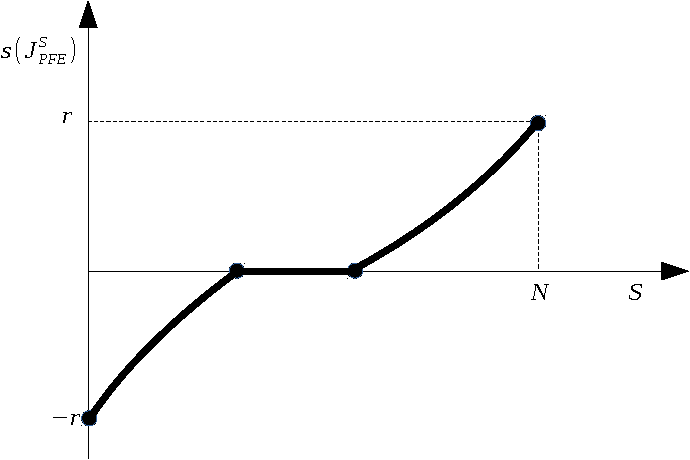
\includegraphics[width=0.49\textwidth]{FIGS/bifurcation_case_interval}
		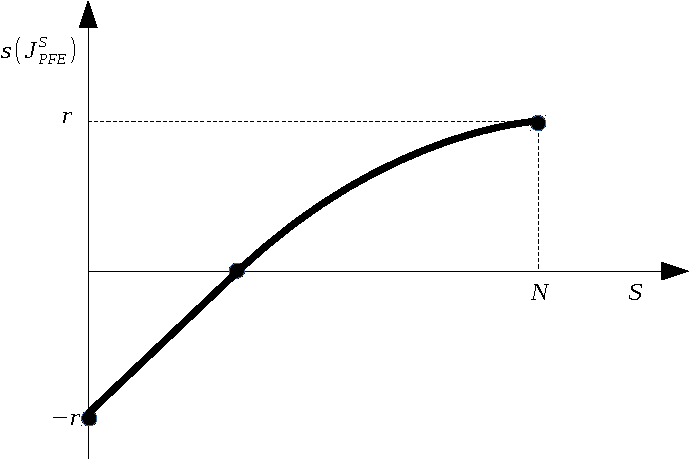
\includegraphics[width=0.49\textwidth]{FIGS/bifurcation_case_unique}
	\end{center}
\end{frame}

\maxFrameImage{FIGS/vary_r_and_S_BA}
\maxFrameImage{FIGS/vary_r_and_S}
\maxFrameImage{FIGS/vary_r_and_S_zoom}

\begin{frame}
	As indicated by \cite{DeutschNeumann1985}, perturbation of the diagonal leads to convex changes in the spectral abscissa on each sub-interval
\end{frame}


\begin{frame}{We have a reproduction number when $\M$ irreducible}
	\begin{proposition}\label{prop:R0}
		Suppose the movement matrix $\M$ is irreducible. 
		Define the basic reproduction number
		\begin{equation}\label{eq:R0}
			\R_0 = \rho\left(
			\left(\M_s+\M_{st}(\D_t-\M_{t})^{-1}\M_{ts}\right)^{-1}\D_s
			\right)
		\end{equation}
		where $\M_s,\M_t,\M_{st},\M_{ts}$ are defined as in \eqref{eq:M_blocks}, $\D_s$ and $\D_t$ are defined as in Section~\ref{sec:LAS_PFE}
		Then
		\begin{equation}
			s(J_{\textrm{PFE}}^S)<0 \iff \R_0<1 \textrm{ and }
			s(J_{\textrm{PFE}}^S)>0 \iff \R_0>1
		\end{equation}
	\end{proposition}
\end{frame}

\begin{frame}{Proof of Proposition~\ref{prop:R0}}
		Write \eqref{eq:J_PFE} as
		\[
		J_{\textrm{PFE}}^S=\M+\tilde\D_s-\tilde D_t
		\]
		where $\tilde\D_s=\D_s\oplus\b0_{N-S\times N-S}$ and $\tilde \D_t=\b0_{S\times S}\oplus\D_t$.
		Let $-\alpha$ be the spectral abscissa of $\M+\tilde\D_s-\tilde\D_t$. 
		From Proposition~\ref{prop:perturbation_mvtMatrix}(\ref{prop:perturbation_mvtMatrix_D}), there is a vector $\bv\gg \b0$ such that
		\[
		(\M+\tilde\D_s-\tilde\D_t)\bv = -\alpha\bv
		\]
		In other words,
		\[
		\alpha\bv = (\tilde\D_t-\M)\bv-\tilde\D_s\bv
		\]
		By the assumption of irreducibility of $\M$, it follows from Proposition~\ref{prop:perturbation_mvtMatrix}(\ref{prop:perturbation_mvtMatrix_DmM2}) that $\tilde\D_t-\M$ is an irreducible nonsingular M-matrix and $(\tilde\D_t-\M)^{-1}\gg\b0$.
		Then
		\[
		\alpha\left(
		\tilde\D_t-\M
		\right)^{-1}\bv
		=\bv -\left(
		\tilde\D_t-\M
		\right)^{-1}
		\tilde\D_s\bv
		\]
		with the matrix $(\tilde\D_t-\M)^{-1}\tilde\D_s>\b0$. As a consequence, from the Perron-Frobenius Theorem, the spectral radius of $(\tilde\D_t-\M)^{-1}\tilde\D_s$ is an eigenvalue and is associated to a nonnegative eigenvector
\end{frame}
		
\begin{frame}{Proof of Proposition~\ref{prop:R0}}
		Let $\bu$ be such an eigenvector, normalised so that $\bu^T\bv=1$.
		Then
		\[
		\alpha\bu^T
		\left(\tilde\D_t-\M\right)^{-1}\bv =
		\bu^T\bv
		\left(1-
		\rho\left\{\left(\tilde\D_t-\M\right)^{-1}\tilde\D_s\right\}
		\right)
		\]
		Thus
		\[
		\alpha>0 \iff \rho\left\{\left(\tilde\D_t-\M\right)^{-1}\tilde\D_s\right\} <1
		\]
		and
		\[
		\alpha<0 \iff \rho\left\{\left(\tilde\D_t-\M\right)^{-1}\tilde\D_s\right\} >1
		\]
		From the structure of $\tilde\D_s$, the spectral radius of $(\tilde\D_t-\M)^{-1}\tilde\D_s$ is the spectral radius of 
		\[
		\left(\tilde\D_t-\M\right)^{-1}_{[11]}\D_s
		\]
		where $(\tilde\D_t-\M)^{-1}_{[11]}$ is the (1,1) block in $(\tilde\D_t-\M)^{-1}$.
		Writing $\M$ as \eqref{eq:M_blocks}, we have by the formula for the inverse of a $2\times 2$ block matrix that 
		\[
		\left(\tilde\D_t-\M\right)^{-1}_{[11]}=(-\M_s-\M_{st}(\D_t-\M_t)^{-1}\M_{ts})^{-1}
		\]
\end{frame}

\begin{frame}{Proof of Proposition~\ref{prop:R0}}
		Clearly,
		\begin{multline*}
			\rho\left(
			(-\M_s-\M_{st}(\D_t-\M_t)^{-1}\M_{ts})^{-1}\D_s
			\right) \\
			=
			\rho\left(
			(\M_s+\M_{st}(\D_t-\M_t)^{-1}\M_{ts})^{-1}\D_s
			\right)
		\end{multline*}
		giving the result
\end{frame}

\section{Global behaviour}
\begin{frame}{So..}
	we are done!
	\vfill
	.. Are we? The result is only local, can we go further?
\end{frame}

\begin{frame}{System \eqref{sys:simple_model} is cooperative}
	Jacobian of \eqref{sys:simple_model}:
	\begin{equation}\label{eq:Jacobian_anywhere}
	J(\bP_s,\bP_t) = 
	\begin{pmatrix}
	\bG_s'(\bP_s)\bP_s+\bG_s(\bP_s)+\M_s & \M_{st} \\
	\M_{ts} & -\D_t+\M_t
	\end{pmatrix}
	\end{equation}
	where
	\[
	\bG_s'(\bP_s) = \diag \left(-\frac{r_1}{K_1},\ldots,-\frac{r_S}{K_s}\right)
	\]
	\vfill
	Thus
	\[
	J(\bP_s,\bP_t) = \M+ \left((\bG_s'(\bP_s)\bP_s+\bG_s(\bP_s))\oplus -\D_t\right)
	\]
	with
	$\bG_s'(\bP_s)\bP_s+\bG_s(\bP_s)$ and $-\D_t$ diagonal
	\vfill
	$\implies$ system \eqref{sys:simple_model} is cooperative
\end{frame}


\begin{frame}{A theorem of Hirsch}
	So, to move forward, we would like to apply the following result
	\vfill
	\begin{theorem}[Th. 6.1 in Hirsch (1984) -- BAMS 11(1)]
		Let $\bF$ be a $C^1$ vector field in $\IR^n$ with flow $\phi$ preserving $\IR_+^n$ for $t>0$ and strongly monotone in $\IR_+^n$. 
		Suppose that the origin is an equilibrium and all trajectories in $\IR_+^n$ are bounded. Suppose the matrix-valued map $D\bF:\IR_+^n\to \IR^{n\times n}$ is strictly antimonotone, i.e., 
		\[
		\bx>\by\implies D\bF(\bx)<D\bF(\by)
		\]
		\vskip0.5cm
		Then either all trajectories in $\IR_+^n$ go to the origin, or there exists a unique equilibrium $\bP^\star\in\mathsf{Int}\IR_+^n$ and all trajectories in $\IR_+^n\setminus\{\b0\}$ limit to $\bP^\star$
	\end{theorem}
\end{frame}

\begin{frame}{OK, nice, but..}
	Take
	\[
	\bP_1 = (0,\ldots,0,\star,\ldots,\star) \textrm{ and }
	\bP_2 = (0,\ldots,0,\star,\ldots,\star)
	\]
	have their first $S$ entries zero, i.e., $\bP_1=(\b0_s,\bP_t^1)$ and $\bP_2=(\b0_s,\bP_t^2)$; assume $\bP_1>\bP_2$, i.e., $\bP_t^1>\bP_t^2$
	\vfill
	Then
	\begin{align*}
	J(\b0_s,\bP_t^1) &= \M+ \left((\bG_s'(\b0_s)\b0_s+\bG_s(\b0_s))\oplus -\D_t\right) \\
	&= \M+\left(\D_s\oplus -\D_t\right) \\
	&= J(\b0_s,\bP_t^2)
	\end{align*}
	i.e.,
	\[
	J^S_{\bP_1}=J^S_{\bP_2}
	\]
	\vfill
	$\implies$ \eqref{sys:simple_model} is not strictly antimonotone
\end{frame}


\begin{frame}{(non) lasciate ogne sperenza, voi ch'intrate}
	Except for strict antimonotonicity of $\bF$, all hypotheses of [Hirsch (1984) -- Th. 6.1] are satisfied:
	\begin{itemize}
		\item in the case $\M$ irreducible, \eqref{sys:simple_model} is strongly monotone (by [Hirsch (1984) -- Th. 1.7])
		\item the origin is an equilibrium
		\item all solutions of \eqref{sys:simple_model} are bounded in $\IR_+^N$
	\end{itemize}
	\vfill
	$\implies$ by other results (\emph{e.g.}, Hirsch \emph{ibid}), there exists $\bP^*\gg \b0$
	\vfill
	What is the use of strict antimonotonicity in the proof of [Hirsch (1984) -- Th. 6.1]? .. To show uniqueness of $\bP^*$
\end{frame}

\begin{frame}
		More precisely: let $\bz\in(\b0,\bP^*)$, where $\bP^*\gg\b0$ is a nontrivial equilibrium
		\vfill
		Strict antimonotonicity $\implies$ $\bF(\bz)>\b0$, and we can then proceed with the remainder of the proof of [Hirsch (1984) -- Th. 6.1]
		\vfill
		Let us show that we indeed have $\bF(\bz)>\b0$ for \eqref{sys:simple_model}, despite the lack of strict antimonotonicity
		\vfill
		As in [Hirsch (1984) -- Th. 6.1]: for $i = 1,\ldots,N$, let 
		\begin{align*}
		g_i :  [0,1] &\to\IR \\
		s &\mapsto F_i(s\bP^*)
		\end{align*}
\end{frame}

\begin{frame}
	Then $g_i(0)=g_i(1)=0$ for $i=1,\ldots,N$ and, for $i=S+1,\ldots,N$ 
	(sinks),
		\[
		g_i(s) = -r_isP_i^*+\sum_{j=1}^Nm_{ij}sP_j^*
		= \left(r_iP_i^*+\sum_{j=1}^Nm_{ij}P_j^*\right)s=0
		\]
		However, for $i=1,\ldots,S$ (sources),
		\[
		g_i(s) = r_i\left(1-\frac{sP_i^*}{K_i}\right)sP_i^*
		+\sum_{j=1}^Nm_{ij}sP_j^*
		\]
		Ha!
		\[
		g_i''(s)=-\frac{2r_iP_i^{*2}}{K}<0,\quad i=1,\ldots,S
		\]
		\vfill
		$\implies$ for $i=1,\ldots,S$, $g_i(s)>0$ when $s\in(0,1)$
		
		$\implies$ 
		when $S>0$, $\bF(\bz)>\b0$, $\forall\bz\in(\b0,\bP^*)$
		
\end{frame}
		
\begin{frame}
	And we can then carry on with the remainder of the proof of [Hirsch (1984) -- Th. 6.1]
	\vfill
	To finish, the case $S=0$ is easy: 
	\[
	\left(\sum_{i=1}^{N}{P_i}\right)' 
	= -\sum_{i=1}^N r_iP_i < 0
	\]
	since at least one of the $P_i(0)>0$ 
	\vfill 
	$\implies$ $\left(\sum_{i=1}^{N}{P_i}\right)\to 0$ $\implies$ $\lim_{t\to\infty}P_i(t)=0$ for $i=1,\ldots,N$
	\vfill
	Et hop! $\square$
\end{frame}

\begin{frame}{To conclude (mathematically)}
	\begin{theorem}\label{th:main_result}
		There exists a critical \emph{interval} $\S_{int}\subset(0,N)\subset\IR$ s.t.
		\begin{itemize}
			\item $S<\min(\S_{int})$ $\implies$ PFE LAS
			\item $S>\max(\S_{int})$ $\implies$ PFE instable
		\end{itemize}
		\vskip0.5cm
		Additionally, if the patch digraph is strongly connected, then
		\begin{itemize}
			\item $\S_{int}$ is reduced to a \emph{point}  $S^c$
			\item $S<S^c$ $\implies$ PFE GAS
			\item $S>S^c$ $\implies$ $\exists!\bP^*\gg\b0$ GAS for $\IR_+^N\setminus\{\b0\}$
		\end{itemize}
	\end{theorem}
\end{frame}



%%%%%%%%%%%%%%%%%%%
%%%%%%%%%%%%%%%%%%%
%%%%%%%%%%%%%%%%%%%
%%%%%%%%%%%%%%%%%%%
\section{An interesting special case}
\begin{frame}
	In the 2 figures that follow:
	\begin{itemize}
		\item $N=50$
		\item $r=r_i$, $\forall i=1,\ldots,N$
		\item $m_{ij}=m$, $\forall i,j=1,\ldots,N$ s.t. $m_{ij}>0$
		\item plot is value of $S^c$ as a function of $m$ and $r$
	\end{itemize}
	\vfill
	Figure 1: ring of patches
	\vfill
	Figure 2: complete digraph
\end{frame}


\maxFrameImage{FIGS/Sc_vs_r_and_m_ring}
\maxFrameImage{FIGS/Sc_vs_r_and_m_complete}

\begin{frame}{Case of complete homogeneous movement}
	\begin{proposition}\label{prop:Sc_mvt_complete_homog}
		Suppose that the movement digraph is complete and that $m_{ij}=m$ for $i,j=1,\ldots,N$, $i\neq j$
		\vskip0.2cm
		Suppose that $S\in\{1,\ldots,N-1\}$, that for $i=1,\ldots,S$, $r_i=r_s$ and that for $i=S+1,\ldots,N$, $r_i=r_t$
		\vskip0.2cm
		Then
		\begin{equation}\label{eq:Sc_mvt_complete_homog}
		S^c = \frac{mNr_t-r_sr_t}{m(r_s+r_t)}
		\end{equation}
	\end{proposition}
	\vfill
	If $r_s=r_t=r$, then
	\begin{equation}\label{eq:Sc_mvt_complete_homog_equal_r}
	S^c=\frac N2-\frac{r}{2m}
	\end{equation}
\end{frame}

\maxFrameImage{FIGS/Sc_vs_rs_and_rt_complete}
	
\begin{frame}{Proof of Prop~\ref{prop:Sc_mvt_complete_homog} uses equitable partitions}
	Section 9.3 in \emph{Algebraic Graph Theory}, Godsil \& Royle (2013) 
	\vfill
	An \textbf{equitable partition} $\pi$ splits a graph $X$ into \textbf{cells} $\C_i$, $i=1,\ldots,r$, s.t. for a vertex $u$ in cell $\C_i$, the number of neighbours in cell $\C_j$ is a constant $b_{ij}$ that does not depend on $u$ 
	\vfill
	$\iff$ the subgraph of $X$ induced by each cell is regular [vertices have same degree] and edges joining two distinct cells form a semiregular bipartite graph [vertices have same degree in each bipartite component]
	\vfill
	The digraph with the $r$ cells of $\pi$ as vertices and the $b_{ij}$ arcs from the $i^{\textrm{th}}$ to the $j^{\textrm{th}}$ cell of $\pi$ is the \textbf{quotient} $X/\pi$ of $X$ on $\pi$. The adjacency matrix of $X/\pi$ is $A(X/\pi)=[b_{ij}]$
\end{frame}

\begin{frame}{Characterising an equitable partition}
\begin{lemma}[A friendly characterisation]
	$X$ graph, $A(X)$ its adjacency matrix, $\pi$ a partition of $V(X)$ with characteristic matrix $P$. Then
	\begin{center}
		$\pi$ equitable $\iff$ column space of $P$ is $A$-invariant
	\end{center}
\end{lemma}
\end{frame}

\begin{frame}
	Write
	\begin{equation}\label{eq:J_PFE_equi_part}
	J_{\textrm{PFE}}^S = \begin{pmatrix}
		m\IJ - Nm\II + r_s\II & m \IJ \\
		m\IJ & m\IJ - Nm\II - r_t\II
	\end{pmatrix}
	\end{equation}
	with $\IJ$ matrix of all 1's
	\vfill
	Consider \eqref{eq:J_PFE_equi_part} as the adjacency matrix of a digraph $\G$
	\vfill
	Suppose partition $\pi$ splits $\G$ in two cells, $\{S_i\}_{i=1,\ldots,S}$ (sources) and $\{T_i\}_{i=S+1,\ldots,N}$ (sinks)
	\vfill
	The characteristic matrix of $\pi$ is the $N\times 2$-matrix
	\[
		C = 
		\begin{pmatrix}
		\11_S & \b0_S \\
		\b0_{N-S} & \11_{N-S}
		\end{pmatrix}
	\]
\end{frame}

\begin{frame}
	We have
	\[
		J_{\textrm{PFE}}^S \11 = 
		J_{\textrm{PFE}}^S\begin{pmatrix}
		\11_S\\ \11_{N-S}
		\end{pmatrix}=
		\begin{pmatrix}
		r_s \11_S \\
		-r_t \11_{N-S}
		\end{pmatrix}
	\]
	\vfill
	Thus the column space of $C$ is $J_{\textrm{PFE}}^S$-invariant $\implies$ $\pi$ is equitable
\end{frame}

\begin{frame}{Properties of equitable partitions}
\begin{lemma}
	$\pi$ equitable partition of graph $X$ with characteristic matrix $P$, and $B=A(X/\pi)$. Then $AP = PB$ and
	$B=(P^TP)^{-1}P^T AP$
\end{lemma}
\vfill
\begin{theorem}
	$\pi$ equitable partition of graph $X$ $\implies$ characteristic polynomial of $A(X/\pi)$ divides characteristic polynomial of $A(X)$
\end{theorem}
\end{frame}

\begin{frame}
	$\implies$ the quotient matrix $B_{\textrm{PFE}}^S$ satisfies
\[
B_{\textrm{PFE}}^S = (C^TC)^{-1}C^TJ_{\textrm{PFE}}^SC
\label{eq:formulaJPPB}
\]

\[
\implies B_{\textrm{PFE}}^S = \begin{pmatrix}
mS - mN +r_s & m(N-S) \\
mS & -(mS + r_s)
\end{pmatrix}
\]
\vfill
And $\sigma(B_{\textrm{PFE}}^S) \subset \sigma(J_{\textrm{PFE}}^S)$
\end{frame}

\begin{frame}
	$B_{\textrm{PFE}}^S$ essentially nonnegative (and clearly irreducible)
	\[
	\implies\exists! \bv_p\gg \b0 
	\textrm{ s.t. }  B_{\textrm{PFE}}^S\bv_p = \lambda_p \bv_p=s(B_{\textrm{PFE}}^S)\bv_p
	\]
	\vfill 
	Then $J_{\textrm{PFE}}^SC=CB_{\textrm{PFE}}^S$
	\vfill
	So
	\begin{equation*}
		J_{\textrm{PFE}}^SC\bv_p = CB_{\textrm{PFE}}^S\bv_p = \lambda_p C \bv_p
	\end{equation*}
	and $C\bv_p$ is an eigenvector of $J_{\textrm{PFE}}^S$ that is also $\gg\b0$
	\vfill
	As the only eigenvector $\gg\b0$ of $J_{\textrm{PFE}}^S$ corresponds to $s(J_{\textrm{PFE}}^S)$, we have $s(J_{\textrm{PFE}}^S) = s(B_{\textrm{PFE}}^S)$ 
\end{frame}

\begin{frame}	
	To compute $S^c$, recall $S^c$ is value of $S$ where PFE loses stability
	\vfill
	Consider $B_{\textrm{PFE}}^S$. We have $\tr(B_{\textrm{PFE}}^S) = -mN +r_s-r_t$ and
	\[
		\det(B_{\textrm{PFE}}^S) = -mS(r_s+r_t) - r_sr_t  + mNr_t
	\]
	\vfill
	One shows easily that $\det(\cdot)$ gouverns stability
	\vfill
	\[
		\implies S^c = \frac{mNr_t-r_sr_t}{m(r_s+r_t)}
	\]
	\flushright$\square$
\end{frame}


\bibliographystyle{apalike}
\bibliography{math,biblio_Arino_Julien,ecology}


\end{document}
